\documentclass[a4paper]{scrartcl}

\usepackage[
typ=ib,
fach=Mathematik,
lerngruppe=2BF,
farbig,
namensfeldAnzeigen,
datumAnzeigen,
seitenzahlen = auto,
loesungen = keine,
module= {Papiertypen}
]{schule}

\usepackage{float}
\usepackage{amsmath}

\usepackage[]{fourier-otf}
\usepackage{microtype}	
\author{Maximilian Hertenstein}
\date{\today}
\title{Parallele Geraden}
\date{Datum: \hspace{1.5cm}}

\usepackage{tkz-base}
\usepackage{tkz-fct}
\ifoot{% TODO: \usepackage{graphicx} required

		
\includegraphics[width=0.2\linewidth]{GHSE-Logo}

}

\begin{document}

\section*{Parallele Geraden}

\subsection*{Geraden mit verschiedener Steigung}
$$f\colon y= 3x -5 \qquad g\colon y= 2x -3$$

\begin{minipage}{0.5\linewidth}
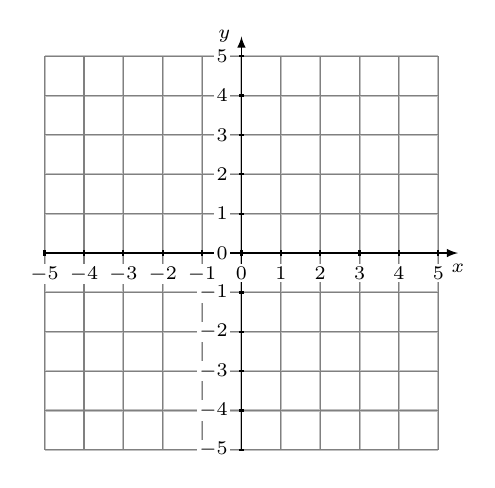
\begin{tikzpicture}[scale = 0.5]
	\scriptsize
	\tkzInit[ymax=5, xmax=5, xmin=-5, ymin=-5, xstep=1, ystep=1]
	\tkzGrid[sub,subxstep=1,subystep=1]
	\begin{scope}
	\tkzFct[samples=50,domain=-5:5,color=blue]{3*x-5}
	\tkzFct[samples=50,domain=-5:5,color=red]{2*x-3}
	\end{scope}
	\color{black}
	\tkzAxeXY[/tkzdrawX/label=$x$,/tkzdrawY/label=$y$]
\end{tikzpicture}
\end{minipage}
\hfill
\begin{minipage}{0.56\linewidth}
\small\renewcommand{\arraystretch}{1.2}
\textbf{$f$}\\[0.5mm]
\begin{tabular}{|c|c|c|c|c|c|c|}
\hline
$x$ & $-1$ & $0$ & $1$ & $2$ & $3$ & $4$ \\
\hline
$y$ & $-8$ & $-5$ & $-2$ & $1$ & $4$ & $7$ \\
\hline
\end{tabular}

\medskip
\textbf{$g$}\\[0.5mm]
\begin{tabular}{|c|c|c|c|c|c|c|}
\hline
$x$ & $-1$ & $0$ & $1$ & $2$ & $3$ & $4$ \\
\hline
$y$ & $-5$ & $-3$ & $-1$ & $1$ & $3$ & $5$ \\
\hline
\end{tabular}

\medskip
\textbf{Abstand}\\[0.5mm]
\begin{tabular}{|c|c|c|c|c|c|c|}
\hline
$x$ & $-1$ & $0$ & $1$ & $2$ & $3$ & $4$ \\
\hline
$d$ & $3$ & $2$ & $1$ & $0$ & $1$ & $2$ \\
\hline
\end{tabular}
\end{minipage}

\medskip
Vor dem Schnittpunkt nimmt der Abstand ab, im Schnittpunkt ist er $0$, danach nimmt er wieder zu.
\subsection*{Geraden mit gleicher Steigung}
$$f\colon y= 2x -5 \qquad g\colon y= 2x -3$$

\begin{minipage}{0.5\linewidth}
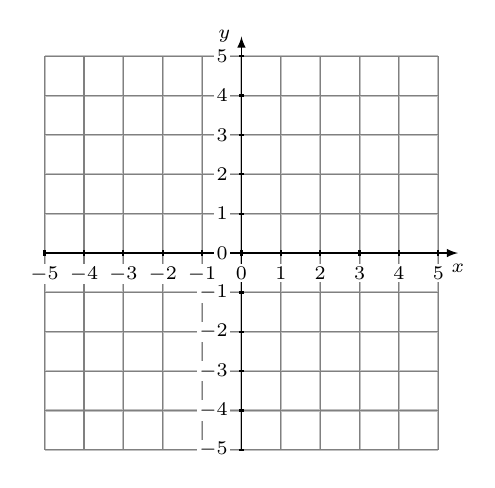
\begin{tikzpicture}[scale = 0.5]
	\scriptsize
	\tkzInit[ymax=5, xmax=5, xmin=-5, ymin=-5, xstep=1, ystep=1]
	\tkzGrid[sub,subxstep=1,subystep=1]
	\begin{scope}
	\tkzFct[samples=50,domain=-5:5,color=blue]{2*x-5}
	\tkzFct[samples=50,domain=-5:5,color=red]{2*x-3}
	\end{scope}
	\color{black}
	\tkzAxeXY[/tkzdrawX/label=$x$,/tkzdrawY/label=$y$]
\end{tikzpicture}
\end{minipage}
\hfill
\begin{minipage}{0.56\linewidth}
\small\renewcommand{\arraystretch}{1.2}
\textbf{$f$}\\[0.5mm]
\begin{tabular}{|c|c|c|c|c|c|c|}
\hline
$x$ & $-1$ & $0$ & $1$ & $2$ & $3$ & $4$ \\
\hline
$y$ & $-7$ & $-5$ & $-3$ & $-1$ & $1$ & $3$ \\
\hline
\end{tabular}

\medskip
\textbf{$g$}\\[0.5mm]
\begin{tabular}{|c|c|c|c|c|c|c|}
\hline
$x$ & $-1$ & $0$ & $1$ & $2$ & $3$ & $4$ \\
\hline
$y$ & $-5$ & $-3$ & $-1$ & $1$ & $3$ & $5$ \\
\hline
\end{tabular}

\medskip
\textbf{Abstand}\\[0.5mm]
\begin{tabular}{|c|c|c|c|c|c|c|}
\hline
$x$ & $-1$ & $0$ & $1$ & $2$ & $3$ & $4$ \\
\hline
$d$ & $2$ & $2$ & $2$ & $2$ & $2$ & $2$ \\
\hline
\end{tabular}
\end{minipage}

\medskip
Der Abstand ist immer $2$ und wird nie $0$. Die Geraden haben keinen Schnittpunkt.


\subsection*{Merke}

\fbox{\parbox{0.9\linewidth}{%
Geraden mit \textbf{gleicher Steigung} und \textbf{verschiedenem $y$-Achsenabschnitt} schneiden sich nie.\\[1mm]
Geraden mit \textbf{verschiedener Steigung} schneiden sich in genau einem Punkt.}}

\end{document}
